%%%%%%%%%%%%%%%%%%%%%%%%%%%%%%%%%%%%%%%%%%%%%%%%%%%%%%%%%%%%%%%%%%%%%%%%%%%
%
% Plantilla para un artículo en LaTeX en español.
%
%%%%%%%%%%%%%%%%%%%%%%%%%%%%%%%%%%%%%%%%%%%%%%%%%%%%%%%%%%%%%%%%%%%%%%%%%%%

% Qué tipo de documento estamos por comenzar:
\documentclass[a4paper]{article}
% Esto es para que el LaTeX sepa que el texto está en español:
\usepackage[spanish]{babel}
\selectlanguage{spanish}
% Esto es para poder escribir acentos directamente:
\usepackage[utf8]{inputenc}
\usepackage[T1]{fontenc}



%% Asigna un tamaño a la hoja y los márgenes
\usepackage[a4paper,top=3cm,bottom=2cm,left=3cm,right=3cm,marginparwidth=1.75cm]{geometry}

%% Paquetes de la AMS
\usepackage{amsmath, amsthm, amsfonts}
%% Para añadir archivos con extensión pdf, jpg, png or tif
\usepackage{graphicx}
\graphicspath{ }
\usepackage[colorinlistoftodos]{todonotes}
\usepackage[colorlinks=true, allcolors=blue]{hyperref}

%% Primero escribimos el título
\title{Contribución a la teoría \\ de \\ comparaciones por pares }
\author{Daniel Cerezo García\\ Inmaculada García Moreno \\ Julián Garrido Arana \\ Juan Valentín Guerrero Cano \\ Cristina Marín Re \\
	
  \small Universidad de Granada \\ UGR
  
  \date{}
}

%% Después del "preámbulo", podemos empezar el documento

\begin{document}
%% Hay que decirle que incluya el título en el documento
\maketitle
\begin{center}

\includegraphics{ugr}\\
\end{center}

\begin{abstract}
Artículo que relaciona la contribución a la Teoría de Comparación por Pares realizada por parte de M.G.Kendall en 1955 y el Algoritmo de Pagerank
\end{abstract}

\section{Introducción}
	Nuestro trabajo ha consistido en la búsqueda de un artículo, la lectura y comprensión del mismo, y por último, la explicación resumida de su desarrollo junto con la relación con conceptos trabajados en la asignatura de Modelos Matemáticos I, concretamente, Page-Rank.\\
	

	Hemos escogido un artículo que trata el problema de las comparaciones mediante pares en un conjunto de N objetos o situaciones para decidir un ranking (ordenación) de los mismos. A lo largo del artículo, se explican diversos métodos y criterios, plasmados a través de ejemplos concretos (p.e. torneos de ajedrez) para determinar la mejor forma en cada caso (según el criterio escogido) de determinar dicho ranking.\\
	

	Introduzcamos pues el artículo:\\
	

	En primer lugar, veamos en qué consiste exactamente la comparación mediante pares (“paired-comparison”) de objetos: Al comparar dos objetos entre sí (comparación de un par), vemos que la relación que se da entre ellos es que uno es preferible sobre otro (según estipule el criterio escogido). Llamemos a uno, sea el objeto A, “\textit{objeto preferible}” y al otro, sea el objeto B, “\textit{objeto no preferible}”. Y expresemos esta relación entre ambos como $A > B$.\\
	

	Vemos en primer lugar que si tenemos tres objetos: A, B y C  y los comparamos entre sí dos a dos de forma que $A > B$ y $B > C$ , cabe esperar entonces que siguiendo la estructura transitiva de un ranking, $A > C$. Sin embargo, puede ocurrir que con el criterio de comparación escogido, al realizar la comparación del par AC, $C > A$. Esto implica que la comparación a pares de N objetos sirve para estipular finalmente un ranking de todos ellos (habiendo hecho todas las comparaciones necesarias como veremos más adelante), pero no tiene por qué seguir una estructura transitiva de por si.\\
	

	\textbf{Ejemplo 1 (propio)} :
	Si tenemos un torneo deportivo en el que participan tres equipos: Equipo A, equipo B y equipo C y todos se enfrentan entre sí una vez de forma que el equipo A gana al equipo B y el equipo B gana al C. Esto no implica directamente que el equipo A gane al C, si no que puede ocurrir que el equipo C gane al A.\\
	

	Como ya hemos mencionado, este tipo de comparaciones siguen un criterio concreto, que siempre es determinista en cuanto al objeto preferible, pero que no ha de ser obligatoriamente objetivo. Veamos esto con claridad en un ejemplo. \\
	

	\textbf{Ejemplo 2 (propio)}:
	Si tenemos un conjunto de 6 sabores de helado diferentes, y tres jueces (críticos culinarios) dispuestos a decidir qué sabores son los mejores pudiendo elegir cada uno tres de los seis sabores como elegidos, y teniendo el voto de cada uno el mismo peso (igual importancia), puede ocurrir lo siguiente: \\
	
	Llamemos a los jueces 1, 2 y 3. El resultado de la votación es que las elecciones de 1 y 2 coinciden exactamente, y difieren por completo de la votación de 3. Por tanto, el resultado final de la cata será que los tres mejores sabores son los escogidos por 1 y 2 y que por tanto, las preferencias de 3, acaban siendo despreciadas (sin repercusión).\\
	

	En este ejemplo anterior ya hemos visto factores importantes a la hora de una comparación como puede ser el peso de cada voto o acción de los distintos representantes en un criterio de elección. Entonces, es importante el diseño del modelo de elección y/o votación a la hora de afrontar estos procesos de ranking y comparación. A lo largo del trabajo veremos más factores de este tipo y valoraremos también muchos otros como las votaciones múltiples, ordenadas*, con número de votos variable, etc. En definitiva, estudiaremos su repercusión en este modelo (comparación y Page-Rank). \\
	

	* Entendemos como votación ordenada, aquella en la que importa el orden de selección cuando se debe votar como elegidos más de un objeto o representante.\\
	

	Veamos una última situación introductoria:\\
	

	\textbf{Ejemplo 3 (artículo)}:
	Imaginemos que en un país se realiza una votación para elegir al próximo presidente, y cada ciudadano tiene que otorgar un voto a uno de los dos candidatos que se presentan: A y B. Todo ciudadano vota y el resultado es que el 51$\%$ de la población elige al candidato A y el 49$\%$ restante al candidato B. Por consiguiente, como el criterio declara como vencedor al que consiga mayor número de votos, se le otorga la presidencia a A. De esta manera, el 51$\%$ de las preferencias quedan satisfechas pero sin embargo un 49$\%$ de las mismas son violadas debido al sistema de la votación.\\
	

	De forma general, a la hora de realizar una elección entre una serie de candidatos, en la mayoría de los casos no se va a lograr obtener una completa unanimidad, luego se tendrán que violar una serie de preferencias. Así pues, el objetivo será minimizarlas.\\
	
	
\section{Teoría de comparación por pares}
	Como ya hemos comentado, el propósito del artículo es violar el menor número de preferencias posibles dadas unas votaciones, o hacer una clasificación “\textit{más justa}” dados los resultados de una competición. En el artículo empieza con los resultados de una votación, e intentar llegar a un método que clasifique estos resultados con las condiciones que buscamos.\\
		
		Tenemos un grupo de 7 personas que tienen que votar, de entre ellos, los tres participantes que quieren que formen un tribunal. Supongamos que no pueden votarse entre ellos, que no hay abstenciones y que no los votan en orden si no que los tres votos valen por igual. Imaginemos estos resultados:\\
\begin{center}
A: BDE \\

B: DAF \\

C: DGA\\

D: CBE\\

E: ABC\\

F: ACD\\

G: BAC\\
\end{center}

Vamos a interpretar estos resultados de esta manera: Si A ha votado a B, D y E. A prefiere a B por encima de H, de C y de G. Y lo mismo con D y E. Creamos una tabla 7X7 donde, en la casilla de la fila i x columna j estará el número de miembros que prefieren a la persona i por encima de la persona j. Es decir el número de votaciones  (excepto la de j) en las que aparece la persona i y no la persona j.\\

Haciendo la tabla a mano nos ha quedado así:\\

\hspace{3cm}$\begin{pmatrix}
     & A & B & C & D & E & F & G & \\ \\
   A & - & 2 & 1 & 2 & 4 & 3 & 3 & 15\\ \\
   B & 1 & - & 1 & 2 & 1 & 4 & 3 & 12\\\\
   C & 1 & 1 & - & 2 & 2 & 3 & 3 & 12\\\\
   D & 0 & 2 & 2 & - & 3 & 2 & 3 & 12\\\\
   E & 1 & 0 & 1 & 0 & - & 2 & 2 & 6\\\\
   F & 0 & 0 & 1 & 0 & 1 & - & 1 & 3\\\\
   G & 0 & 1 & 0 & 0 & 1 & 1 & - & 3\\\\
     & 3 & 6 & 6 & 6 & 12 & 15 & 15 & 63\\\\
\end{pmatrix}$\\
\\


	La tabla que sale en el artículo no queda exactamente igual, pero vamos a trabajar con la que aparece en el artículo puesto que los resultados son parecidos.\\
	
\hspace{3cm}$\begin{pmatrix}
     & A & B & C & D & E & F & G & TOTALS\\ \\
   A & - & 2 &   & 3 & 4 & 3 & 3 & 15\\ \\
   B & 1 & - & 1 & 2 & 1 & 4 & 3 & 12\\\\
   C & 1 & 1 & - & 3 & 3 & 3 & 4 & 15\\\\
   D &   & 2 & 1 & - & 2 & 2 & 2 & 9\\\\
   E & 1 &   & 1 &   & - & 2 & 2 & 6\\\\
   F &   &   &   & 1 & 1 & - & 1 & 3\\\\
   G &   & 1 &   &   & 1 & 1 & - & 3\\\\
   TOTALS  & 3 & 6 & 3 & 9 & 12 & 15 & 15 & 63\\\\
\end{pmatrix}$\\
	\\
	
	 El valor que aparece en la última columna es el número de veces que han preferido a ese miembro antes que a otro. Y 63 es el número total de preferencias.
Y dado un miembro, la suma de su fila y su columna siempre da 18 porque, cada uno de los miembros está siendo comparado con otros tres, por los 6 miembros restantes.\\

Si juzgamos por los resultados de esta última columna, los miembros A y C son los que tienen el valor más alto, 15, seguidos del participante B siendo preferido 12 veces antes que otros miembros. El autor del artículo dice “\textit{Como satisfacemos el mayor número de preferencias posibles, y como el número total de preferencias es constante, minimizamos el número de preferencias violadas}”.\\\\


Supongamos ahora que los miembros votan en orden de preferencia, con los mismos votos que antes. Por ejemplo, A habría votado primero B, luego D y por último E. Antes cada elector expresaba 9 preferencias: A prefería a B por encima de CFG, a D por encima de CFG y a E por encima de CFG. Ahora expresa 12 preferencias: a B por encima de DECFG, a D por encima de ECFG y a E por encima de CFG. Ahora obtendríamos la tabla:\\



\hspace{3cm}$\begin{pmatrix}
     & A & B & C & D & E & F & G & TOTALS\\ \\
   A & - & 3 & 3 & 4 & 4 & 4 & 3 & 21\\ \\
   B & 2 & - & 3 & 3 & 3 & 4 & 3 & 18\\\\
   C & 2 & 2 & - & 4 & 4 & 4 & 4 & 20\\\\
   D & 1 & 2 & 1 & - & 3 & 2 & 3 & 12\\\\
   E & 1 & 0 & 1 & 0 & - & 2 & 2 & 6\\\\
   F & 0 & 0 & 0 & 1 & 1 & - & 1 & 3\\\\
   G & 1 & 1 & 0 & 0 & 1 & 1 & - & 4\\\\
   TOTALS  & 7 & 8 & 8 & 12 & 16 & 17 & 16 & 84\\\\
\end{pmatrix}$\\
	\\
	
donde los clasificados serían A, C y B, mirando en la última columna de los resultados finales.\\


	Este método puede ser utilizado para cualquier número de miembros del grupo total y del comité que se quiere formar. Antes pusimos las condiciones de que no puede haber abstenciones, nadie se puede votar a sí mismo, son ellos mismos los que se votan entre ellos… Pero muchas de estas condiciones pueden relajarse: por ejemplo, votarse a sí mismo no afecta en nada al método, puede haber abstenciones, o incluso algún votante puede empatar a algunos de los miembros que vota. En este último caso simplemente ninguno tiene preferencia sobre el otro. También funciona si los que votan son un grupo de personas distintas a las personas votadas. Este sistema propuesto funciona siempre que todos los jueces tengan el mismo número de votos y estos valgan lo mismo. De esta manera hemos construido, dados un sistema de comparación por parejas, un ranking que minimiza el número de preferencias violadas.\\
	

	Kendall comenta ahora que va a “\textit{considerar diversos desarrollos que son necesarios para permitir un estudio más profundo de las situaciones de comparaciones por parejas}”. Para ilustrarlo, utiliza un ejemplo.\\
	

	Supongamos 6 jugadores en un torneo de ajedrez, donde si ganas te asignan 1 punto, si empatas $\dfrac{1}{2}$ y si pierdes, 0. Y plasmémoslo en una tabla, siendo la fila i x columna j el resultado del participante i, en su partida contra el jugador j. En las casillas i x i pondremos $\dfrac{1}{2}$. Esto no afectará en nada al resultado porque cada jugador tendrá simplemente $\dfrac{1}{2}$ más.\\\\
	
\hspace{3cm}$\begin{pmatrix}
     & A & B & C & D & E & F  & Total Score\\ \\
   A & \dfrac{1}{2} & 1 & 1 & 0 & 1 & 1 & 4\cdot\dfrac{1}{2}\\ \\
   B & 0 & \dfrac{1}{2} & 0 & 1 & 1 & 0 & 2\cdot\dfrac{1}{2}\\\\
   C & 0 & 1 & \dfrac{1}{2} & 1 & 1 & 1 & 4\cdot\dfrac{1}{2}\\\\
   D & 1 & 0 & 0 & \dfrac{1}{2} & 0 & 0 & 1\cdot\dfrac{1}{2}\\\\
   E & 0 & 0 & 0 & 1 & \dfrac{1}{2} & 1 & 2\cdot\dfrac{1}{2}\\\\
   F & 0 & 1 & 0 & 1 & 0 & \dfrac{1}{2} & 2\cdot\dfrac{1}{2}\\\\
\end{pmatrix}$\\

	\begin{center}
	TABLA (7)
	\end{center}
	
	En la última columna volvemos a observar la clasificación final de los jugadores. A y C quedaron los primeros, luego B, E y F, y por último D. Si hubiera tres premios de dinero, dividiríamos el primero y segundo entre A y B, y el tercero entre B, E y F. D se quedaría sin premio. Pero, como comenta Kendell, si nos fijamos en las partidas ganadas y perdidas, aunque D sólo haya ganado una partida, le ha ganado la partida al jugador A, que ha quedado el primer clasificado. Es decir, ha ganado al que más partidas había ganado. E incluso A ha ganado a C pero están empatados en el primer puesto. Es el Doctor T.H.Wei. quien, en 1952 en una tesis no publicada, sugiere un método para realizar otra clasificación:\\
	

Se recalcula la puntuación de cada jugador sumando las puntuaciones de cada jugador al que haya ganado y $\dfrac{1}{2}$ de la puntuación del jugador con el que haya empatado. La tabla nos quedaría ahora de esta manera:\\

$
A= \dfrac{1}{2}\cdot(4\cdot\dfrac{1}{2})+ 2\cdot\dfrac{1}{2}+ 4\cdot\dfrac{1}{2} + 0 + 2\cdot\dfrac{1}{2} + 2\cdot\dfrac{1}{2} = 14\cdot\dfrac{1}{4}
$\\

$
B= 0 + \dfrac{1}{2}\cdot(2\cdot\dfrac{1}{2})+ 0 + 1\cdot\dfrac{1}{2} + 2\cdot\dfrac{1}{2} + 0 = 5\cdot\dfrac{1}{4}
$\\

$
C= 0 + 2\cdot\dfrac{1}{2}+ \dfrac{1}{2}\cdot(4\cdot\dfrac{1}{2}) + 1\cdot\dfrac{1}{2} + 2\cdot\dfrac{1}{2} + 2\cdot\dfrac{1}{2} + 2\cdot\dfrac{1}{2} = 11\cdot\dfrac{1}{4}
$\\

$
D= 4\cdot\dfrac{1}{2} + 0 + 0 + \dfrac{1}{2}\cdot(1\cdot\dfrac{1}{2}) + 0 + 0 = 5\cdot\dfrac{1}{4}
$\\

$
E= 0 + 0 + 0 + 1\cdot\dfrac{1}{2} + \dfrac{1}{2}\cdot(2\cdot\dfrac{1}{2}) + 2\cdot\dfrac{1}{2} = 5\cdot\dfrac{1}{4}
$\\

$
F= 0 + 2\cdot\dfrac{1}{2} + 0 + 1\cdot\dfrac{1}{2} + 0 + \dfrac{1}{2}\cdot(2\cdot\dfrac{1}{2}) = 5\cdot\dfrac{1}{4}
$\\

\begin{center}
TABLA (8)
\end{center}
	Ahora las clasificaciones quedan distintas: A queda primero, C segundo, y en tercer lugar el resto empatados. “\textit{¿Y qué pasa si repetimos este procedimiento otra vez?}”, se plantea Kendell. Recalculando la puntuación con el mismo método y los nuevos datos, obtiene \\\\\\\\\\
	
$
A= \dfrac{1}{2}\cdot(14\cdot\dfrac{1}{4})+ 5\cdot\dfrac{1}{4}+ 11\cdot\dfrac{1}{4} + 0 + 5\cdot\dfrac{1}{4} + 4\cdot\dfrac{1}{4} = 34\cdot\dfrac{1}{8}
$\\

$
B= 0 + \dfrac{1}{2}\cdot(5\cdot\dfrac{1}{4})+ 0 + 5\cdot\dfrac{1}{4} + 5\cdot\dfrac{1}{4} + 0 = 13\cdot\dfrac{1}{8}
$\\

$
C= 26\cdot\dfrac{5}{8}
$\\

$
D= 16\cdot\dfrac{7}{8}
$\\

$
E = 13\cdot\dfrac{1}{8}
$\\

$
F= 13\cdot\dfrac{1}{8}
$\\
	
	\begin{center}
TABLA (9)
\end{center}
	Llega un momento en el que al recalcular se obtienen los mismos datos que en el paso anterior, puesto que los valores se estabilizan, logrando así un ranking final, que sería el que podríamos considerar como el más justo, y por tanto, nuestro objetivo es llegar a él.\\
	
	Entonces, Kendell se da cuenta de lo siguiente. Si ponemos la tabla (7) como matriz, nos quedaría así:
	
	\hspace{3cm}$\begin{pmatrix}
     &  &  &  &  &   & Row totals\\ \\
   \dfrac{1}{4} & 3 & 1 & 4 & 2 & 3 & 14\cdot\dfrac{1}{4}\\
   1 & \dfrac{1}{4} & 0 & 2 & 1 & 1 & 5\cdot\dfrac{1}{4} \\\\
   1 & 2 & \dfrac{1}{4} & 4 & 2 & 2 & 11\cdot\dfrac{1}{4}\\\\
   1 & 1 & 1 & \dfrac{1}{4} & 1 & 1 & 5\cdot\dfrac{1}{4}\\\\
   1 & 1 & 0 & 2 & \dfrac{1}{4} & 1 & 5\cdot\dfrac{1}{4}\\\\
   1 & 1 & 0 & 2 & 1 & \dfrac{1}{4} & 5\cdot\dfrac{1}{4}\\\\
\end{pmatrix}$\\
	
	Y si multiplicamos esta matriz por sí misma, es decir, la elevamos al cuadrado, obtenemos una matriz equivalente a la tabla 8. Si tomamos esta matriz resultante y volvemos a multiplicarla por la matriz A, entonces obtenemos los resultados de la tabla 9. Es decir, realizar el proceso propuesto por el doctor T. H. Wei n veces, es equivalente a elevar la matriz A a n. Llegamos a una conclusión muy interesante, y es que la obtención de la matriz formada por los valores estabilizados, es similar a calcular \\
	
\hspace{5cm}$\lim_{n \to \infty}(A^n)$\\

		
		


A continuación, el autor del artículo plantea el problema como un problema de grafos. Suponiendo un caso en el que tenemos n objetos, podemos representar las comparaciones por pares como grafos, en el que cada objeto estará representado por un vértice, y cada comparación estará determinada por una arista, de forma que, si se prefiere al objeto i frente al objeto j, entonces habrá una flecha que vaya del vértice que representa al objeto i, al vértice que representa al objeto j. En el caso de que se determine que no hay preferencia entre un objeto i y uno j, entonces se dibujara una arista no dirigida entre ellos.\\


Como nuestra intención es poder relacionar todos los objetos entre sí, es decir, que se determine la preferencia en todos los pares posibles de objetos, tenemos un grafo completo de n vértices.\\


En el caso del torneo de ajedrez, tendríamos un grafo como el siguiente:\\


\begin{center}
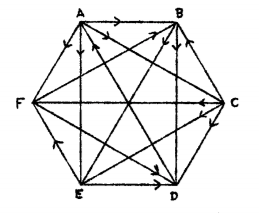
\includegraphics{grafo_completo}\\
\end{center}

Entonces, podemos ver que la tabla 7 puede construirse otorgando a cada vértice, un 1 por cada arista que salga de él, $\dfrac{1}{2}$ por el camino a sí mismo (que no se pinta), y $\dfrac{1}{2}$ por cada arista que pase por el vértice sin tener flecha (los empates). Posteriormente, calculamos para cada vértice, el número de caminos que podemos tomar saliendo de él y dando dos pasos (longitud de camino 2). Asignamos puntuaciones a estos caminos de la misma forma que en el primer paso y los sumamos, obteniendo así la tabla 8. Si volvemos a hacer esto pero con caminos de longitud 3, obtenemos la tabla 9.\\


De nuevo, calcular estas sucesivas tablas a través de los caminos de longitud n, equivale a realizar n veces el método del doctor T.H.Wei o elevar la matriz A a n.\\


Por tanto, como queremos obtener el ranking más justo, al final nuestro objetivo es calcular el límite mencionado anteriormente. Como la matriz A es diagonalizable, este límite va a estar determinado por sus valores propios y, particularmente, por su radio espectral.\\


El estudio de la comparación por pares de la forma explicada, guarda grandes similitudes con el algoritmo de PageRank. Primero, vamos a explicar de qué trata este algoritmo.\\


\section{Algoritmo PageRank}
	Cada vez que un usuario solicita una búsqueda en Google utilizando una frase de búsqueda, el motor de búsqueda determina todas las páginas de la web que contienen las palabras en la frase de búsqueda. El problema es que Google puede tener 25 mil millones de páginas. Por lo que para la mayoría de las búsquedas, habrá una gran cantidad de páginas que contengan las palabras de la frase de búsqueda. Se necesita entonces un algoritmo para clasificar la importancia de las páginas que se ajustan a los criterios de búsqueda para que cuando un usuario busque algo se desplieguen en orden decreciente en función de dicha importancia.
\\

	 La idea fundamental de Page Rank es que la importancia de una página depende tanto del número de páginas que enlazan con ella como del propio valor de las mismas. Vamos a asignar a cada página web P una medida de su importancia F(P), denominada PageRank de la página. Suponemos que cada pagina $P_j$ tiene $l_j$ enlaces de salida. Si uno de esos enlaces apunta a la página $P_i$, entonces $P_j$ va a aportar $\dfrac{1}{l_j}$ de su importancia a $F(P_i)$. Cabe destacar que cada página tiene una importancia inicial. Por lo que el peso o importancia  de una página $P_i$ será:
\\

\hspace{5cm}F($P_i$)=$\sum_{\substack{P_j \in B_i}} \dfrac{S(P_j)}{l_j}$ 
\\

Donde $S(P_j)$ es la importancia inicial de $P_j$. Denotaremos además $B_i$ como el conjunto de páginas que enlazan a $P_i$.
\\

Para aplicar el algoritmo crearemos una matriz H llamada matriz de hiperenlaces, donde a la componente $H_{i,j}$ se le asignará $\dfrac{1}{l_j}$ si existe un enlace de la página $P_j$ a la $P_i$, y 0 en caso contrario.
\\

\hspace{5cm}$H_{i,j}$=$\left\{ \begin{array}{lcc}
             \dfrac{1}{l_j} &   si  & P_j \in B_i \\
             \\ 0 & $ en otro caso$ & 
             \end{array} 
          \right.$
\\

Como se puede apreciar, H es una matriz no negativa, y la suma de cada columna j es igual a 1, siempre y cuando la página $P_j$ tenga  algún enlace de salida. En caso contrario, esta suma será igual a 0. Si toda página $P_j$ tiene enlaces de salida, la matriz H será una matriz estocástica.
\\

	Esta matriz de hiperenlaces la hemos formado con el objetivo de crear un sistema en el que podamos obtener el PageRank de cada página simplemente multiplicando la matriz H por un vector cuyas componentes son las importancias iniciales de las páginas.\\
	
Sabemos que si la matriz H fuera ergódica existiría un vector I que es vector propio de la matriz H con valor propio asociado 1. Lo llamaremos vector estacionario de H, y cumpliría que:

\hspace{5cm}\[ I = H \cdot I 
                \]
\\

Sin embargo, la matriz H no tiene por qué ser ergódica, ya que puede haber columnas cuyas componentes sean todas 0. A las páginas representadas por estas columnas se les llama páginas colgantes. Para resolver este problema, el algoritmo hará que, las páginas que en un principio no referenciaban a ninguna otra, ahora apunten a todas las demás. \\


\textbf{Ejemplo}

Su matriz de hiperenlaces sería primariamente de la siguiente forma:\\


\hspace{5cm}$H^*=\begin{pmatrix}
   0 & \dfrac{1}{3} & 0 & 0 & \dfrac{1}{2} & 0\\\\
   0 & 0 & 1 & 0 & 0 & 0\\\\
   0 & 0 & 0 & 0 & 0 & 0\\\\
   0 & 0 & 0 & 0 & 0 & \dfrac{1}{2}\\\\
   0 & \dfrac{1}{3} & 0 & 0 & 0 & 0\\\\
   0 & \dfrac{1}{3} & 0 & 1 & \dfrac{1}{2} & \dfrac{1}{2}
\end{pmatrix}$\\
\\
\\
\\


Después de resolver el problema de las columnas colgantes quedaría así:\\

\hspace{5cm}$H=\begin{pmatrix}
   \dfrac{1}{6} & \dfrac{1}{3} & 0 & 0 & \dfrac{1}{2} & 0\\ \\
   \dfrac{1}{6} & 0 & 1 & 0 & 0 & 0\\ \\
   \dfrac{1}{6} & 0 & 0 & 0 & 0 & 0\\\\
   \dfrac{1}{6} & 0 & 0 & 0 & 0 & \dfrac{1}{2}\\\\
   \dfrac{1}{6} & \dfrac{1}{3} & 0 & 0 & 0 & 0\\\\
   \dfrac{1}{6} & \dfrac{1}{3} & 0 & 1 & \dfrac{1}{2} & \dfrac{1}{2}
\end{pmatrix}$\\
\\

En nuestro caso, estamos buscando un vector propio de H asociado al valor propio 1. Al ser H una matriz ergódica,  este valor es dominante y, por tanto, menor o igual que cualquier otro valor propio de H. Este vector propio buscado es el vector estacionario nombrado anteriormente. Ahora sí que podemos garantizar su existencia.\\


Ahora el algoritmo se plantea otro problema, y es que hay páginas que solo referencian a una única página, llamadas páginas absorbentes, que pueden restringir la libertad de los usuarios al \textit{surfear} por la web. Por ello, se modifica de nuevo la matriz, para finalmente obtener la conocida como matriz de Google (G).\\

Para hacer esta modificación, se elige un parámetro $\alpha$ entre 0 y 1, y se realiza la operación que sigue para obtener la matriz G:


\hspace{5cm}$G=\alpha \cdot H + \dfrac{(1-\alpha)}{n} \cdot E_n$\\

Donde $E_n$ es la matriz cuadrada de orden n donde todas las celdas tienen valor 1.\\

En nuestro caso, si elegimos $\alpha$= 0.85, la matriz G sería:\\


\hspace{5cm}$G=\begin{pmatrix}
   \dfrac{1}{6} & \dfrac{37}{120} & \dfrac{1}{40} & \dfrac{1}{40} & \dfrac{9}{20} & \dfrac{1}{40}\\ \\
   \dfrac{1}{6} & \dfrac{1}{40} & \dfrac{7}{8} & \dfrac{1}{40} & \dfrac{1}{40} & \dfrac{1}{40}\\ \\
   \dfrac{1}{6} & \dfrac{1}{40} & \dfrac{1}{40} & \dfrac{1}{40} & \dfrac{1}{40} & \dfrac{1}{40}\\\\
   \dfrac{1}{6} & \dfrac{1}{40} & \dfrac{1}{40} & \dfrac{1}{40} & \dfrac{1}{40} & \dfrac{9}{20}\\\\
   \dfrac{1}{6} & \dfrac{37}{120} & \dfrac{1}{40} & \dfrac{1}{40} & \dfrac{1}{40} & \dfrac{1}{40}\\\\
   \dfrac{1}{6} & \dfrac{37}{120} & \dfrac{1}{40} & \dfrac{7}{8} & \dfrac{9}{20} & \dfrac{9}{20}
\end{pmatrix}$\\
\\


Así, si calculamos:

\hspace{5cm}$I_k= G^k \cdot I_0$\\


donde $I_0$ es un vector de importancias iniciales. Pongamos, por ejemplo, que es:\\

\hspace{5cm}$I_0=\begin{pmatrix}
   1 \\
   0 \\
   0 \\
   0 \\ 
   0 \\
   0 \\
\end{pmatrix}$\\\\

Si hiciésemos 500 iteraciones nuestro vector $I_{500}$ quedaría:\\

\hspace{5cm}$I_{500}= G^{500} \cdot I_0$\\

\hspace{5cm}$I_{500}=\begin{pmatrix}
   0.0784 \\
   0.0668 \\
   0.0361 \\
   0.2531 \\ 
   0.0550 \\
   0.5105 \\
\end{pmatrix}$\\

Lo que nos dice que la página más importante es $P_6$ y el PageRank sería:\\

\hspace{5cm}$P_6 < P_4< P_1 < P_2 < P_5 < P_3$\\


\section{Relación entre PageRank y la Teoría de pares comparados}
Como podemos observar en los métodos explicados acerca del artículo, estos tratan de encontrar el ranking más justo dentro un conjunto de objetos según determinados criterios. Esto es, precisamente, lo que resuelve el algoritmo PageRank para establecer la ordenación de un conjunto de páginas web, en base a una importancia que se asigna a cada una.\\


Al igual que en el artículo, en el método de PageRank se puede representar la relación de las páginas a través de los distintos enlaces mediante un grafo dirigido. Además, en ambos casos, usamos el mismo procedimiento para obtener dicho ranking objetivo. Este es elaborar una matriz que represente el grafo mencionado y, a través de un sistema dinámico, determinar la solución con el cálculo de un límite tras una serie de iteraciones. Aquí, los valores propios de las matrices desempeñan también un papel crucial a la hora de determinar la convergencia del sistema.\\


Más profundamente, vemos que en la creación de la matriz se siguen pasos parecidos. En ambos casos, se deben abordar una serie de problemas que surgen a partir de ciertos coeficientes nulos de la matriz. Así, de la misma forma que PageRank resuelve el problema de las páginas colgantes (repartiendo por igual la importancia de las páginas en cuestión), la teoría de pares comparados resuelve un paradigma similar a la hora de evaluar el criterio de comparación de un objeto consigo mismo, de forma que consigue eliminar dichos ceros asignando a cada celda un mismo valor. En los ejemplos vistos del comité o el torneo de ajedrez, esto se aprecia claramente cuando se sustituyen todos los ceros de la diagonal principal de la matriz por 1/2, sin alterar las conclusiones finales del sistema.\\


Finalmente, es destacable mencionar, en particular, la similitud del ejemplo del torneo de ajedrez con PageRank. El método seguido para calcular la importancia de cada página, de forma que tenga en cuenta también la importancia de aquellas con las que está relacionada, es idéntico a cómo se trata el hecho de haber ganado a un jugador más o menos importante en el torneo, en función de las victorias que ha conseguido. Así, si un jugador ha ganado a otro que tiene muchas partidas ganadas, logra más puntuación que otro que, teniendo el mismo número de victorias, son frente a rivales menos valorados. Lo mismo ocurre con las páginas web: si estas son referenciadas por páginas más importantes, conseguirán más estatus en el ranking.\\


\section{Conclusión}
Como conclusión, queremos destacar la importancia de la búsqueda de algoritmos y modelos matemáticos como los estudiados, que clasifiquen un conjunto de objetos para poder tomar decisiones entre ellos. Que teorías separadas por casi medio siglo, busquen soluciones a problemas análogos a través de métodos muy parecidos, refleja cómo esta es una cuestión que seguirá pendiente con el paso del tiempo, debido a la necesidad de encontrar nuevos algoritmos que permitan gestionar y ordenar la gran cantidad de información que se genera actualmente por el avance de las tecnologías (Big Data). De hecho, cabe la posibilidad de que la teoría de pares comparados haya servido como base para determinar el método de PageRank.\\

\section{Referencias}
\textbf{David Austin},\textit{"How Google Finds Your Needle in the Web's Haystack"}, Grand Valley State University, 2013\\

https://www.dam.brown.edu/people/mchb/la/GooglePageRank.pdf\\

\textbf{M. G. Kendall}, \textit{"Further Contributions to the Theory of paired comparisons"}, Institute of Statistics North Caroline State College 1954\\

\bibliographystyle{abbrv}
\bibliography{sample}

\end{document}